\documentclass[a4paper,11pt]{article}
\usepackage[T1]{fontenc}
\usepackage[utf8]{inputenc}
\usepackage{lmodern}
\usepackage[english]{babel}
\usepackage{hyperref}
\usepackage{wrapfig}
\usepackage{graphicx} 

\hypersetup{
  colorlinks   = true, %Colours links instead of ugly boxes
  urlcolor     = blue, %Colour for external hyperlinks
  linkcolor    = black, %Colour of internal links
  citecolor   = black %Colour of citations
}

\title{Design of infrared beacons.}
\author{Matthieu Vigne}

\begin{document}
\maketitle
\tableofcontents
\section{Introduction}

This documents explain the design process and the thinking behind this beacon system. It gives an overall picture of why the beacons were built that way, to help the reader understand how they work, what they output, and how to modify them if desired. This system is still quite in beta, and can surely be improved quite a lot: feel free to do so !

\begin{figure}[h]
  \centering
  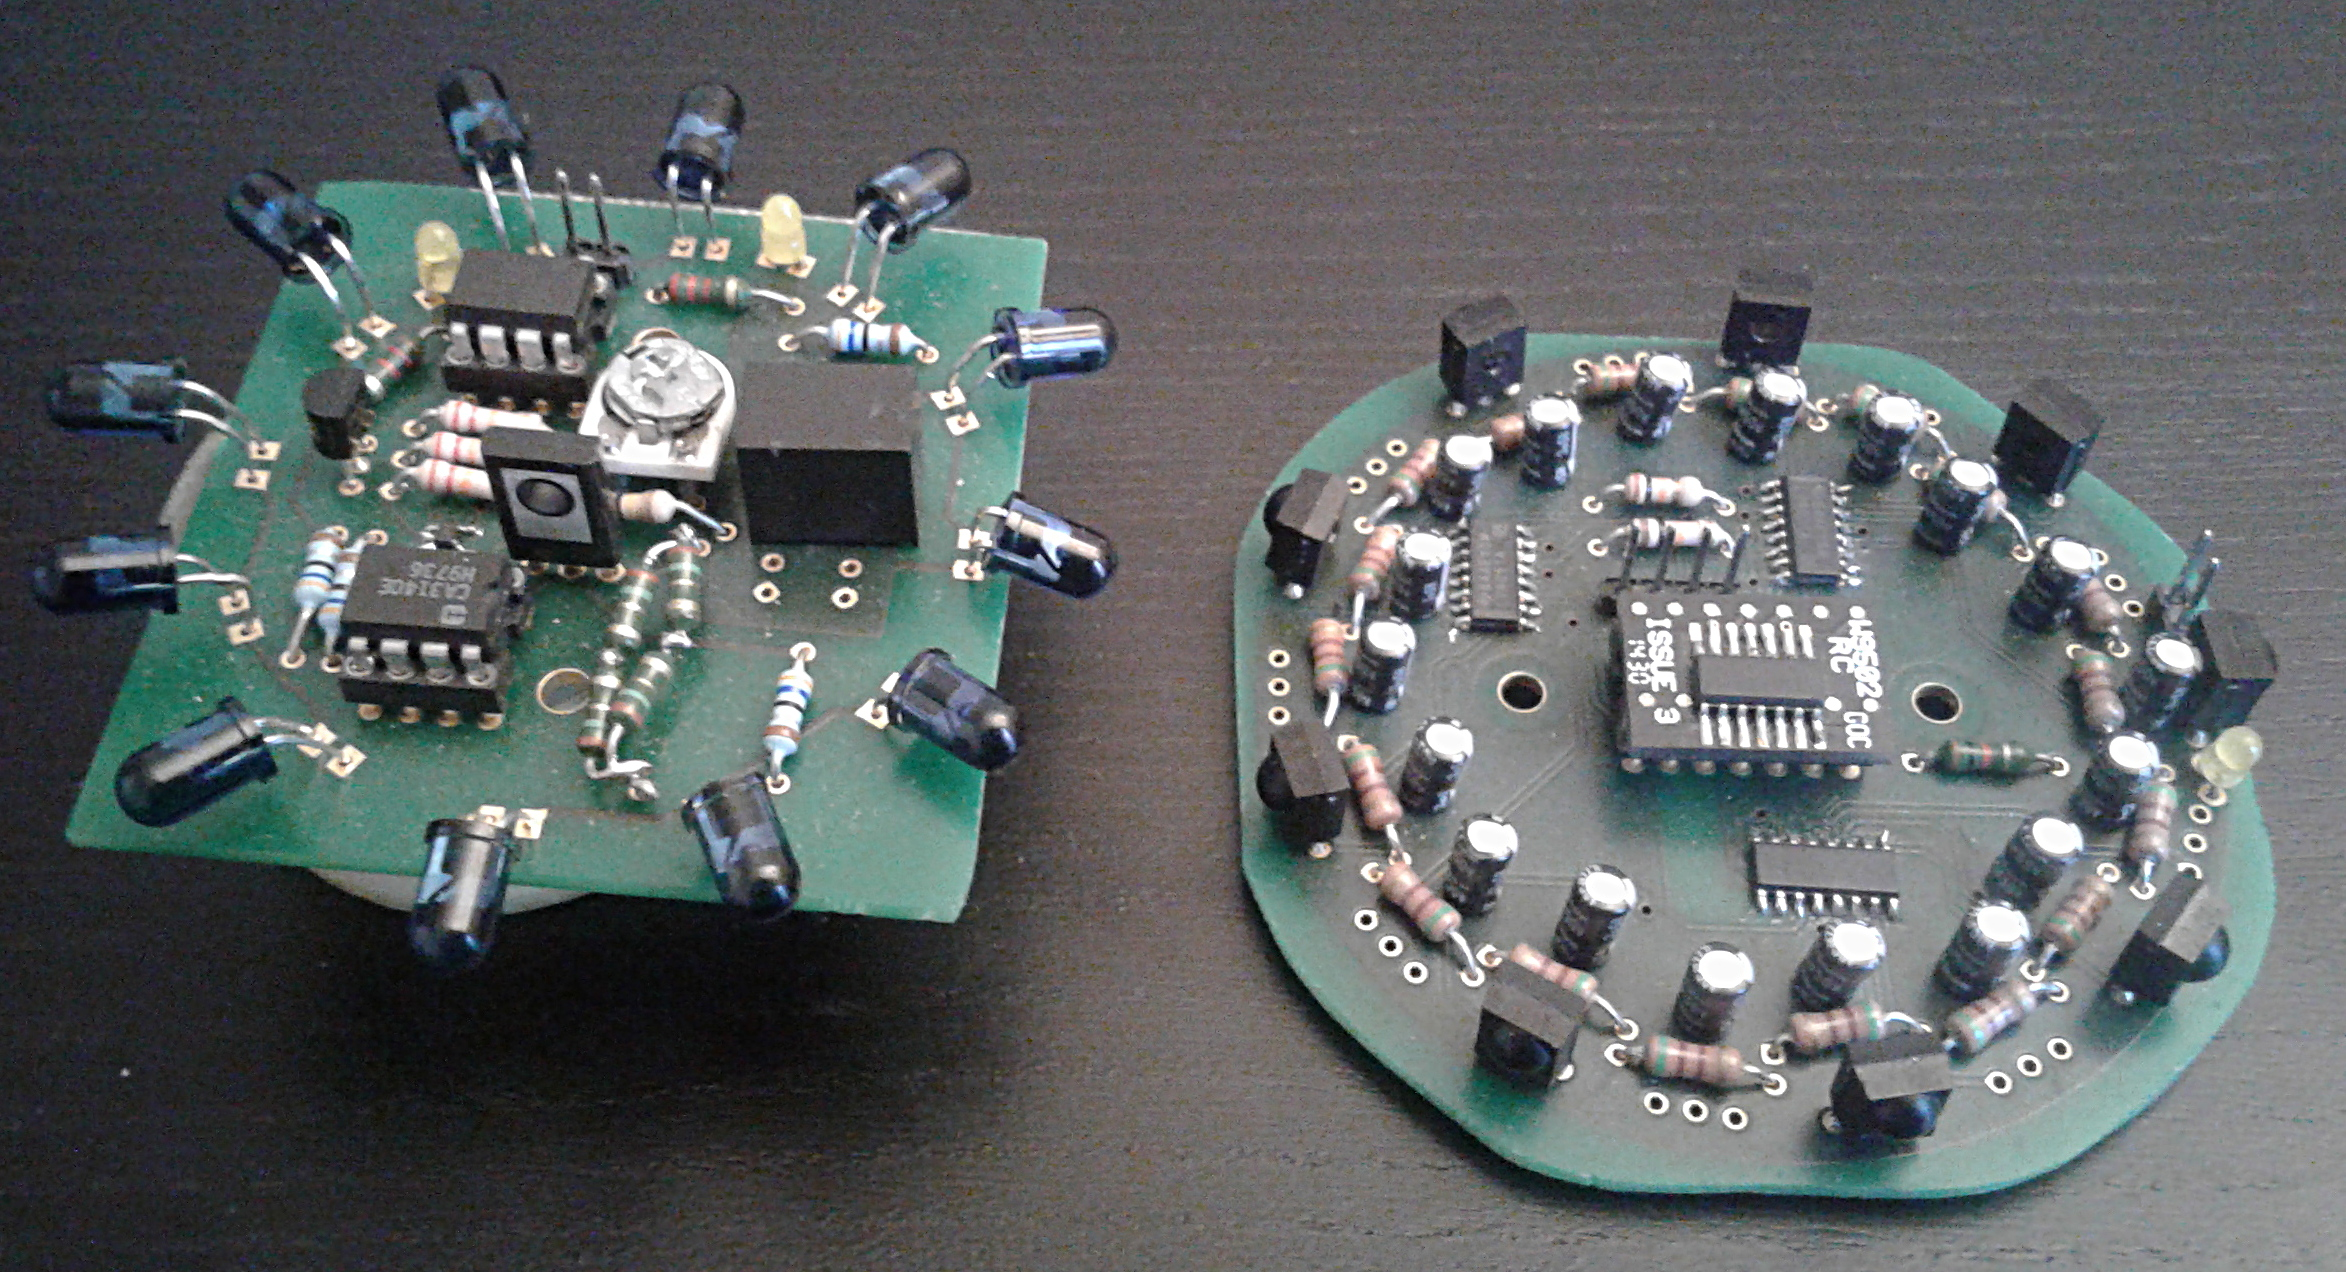
\includegraphics[width=0.8\textwidth]{Figures/Beacons.jpg}
  \caption{Picture of the beacon system: emitter (left) and receiver (right).}
\end{figure}

\section{Working principle}

\subsection{Overview}

The design and key ideas for this beacon originate from the (French) website \href{http://www.totofweb.net/robots-projet-67.html}{totofweb}, which presents a similar design. You might wonder why this work was done, instead of just taking directly the design presented there. The main reason is that it is a bit old, and sadly relies on an obsolete sensor, a TSOP7000 IR sensor. So I started working on a variant, using a different sensor from the same family. Doing this, I also changed the design to match the requirements I wanted.

The principle of IR beacons is to have an emitter on the other robot, sending IR light in all directions, and a belt of IR received on our robot. This receivers are placed such that their field of view overlap, giving 360$360^\circ$ field of view to the robot. I designed it with the following constraints or goals in mind:

 - the receiver and emitter have to fit in an 8x8cm square (the old size of the beacons - in 2018 the size was increased to 10cm and will probably remain that way for the following years, so they could theoretically be bigger now).
 
 - the emitter will work from a 9V battery (this being an easy to use energy source: it can be integrated easily in the size limitation given by Eurobot, and have a longer operating live than, say, small 1.5V/3V batteries).
 
 - the reciever should be as easy to use as possible from the user point of view. As such, individual sensor handling should be done internally, and available data sent back through a serial bus (in this design, I2C, but this can be changed easily).
 
 - sensor reading (and thus detection) should be as fast as possible.
 
 - the receiver should work from 3.3V or 5V source (to work with an Arduino just like a Beaglebone/Raspberry Pi).
 
 - the system should be as robust as possible to external light sources, including light from other beacons (i.e. we still want this to work, even if the other team is using a similar, or completely identical, system). This last point was not treated at all in the Totofweb website.
 
 \subsection{Light source and sensor}

Obviously, the key point in this system is the actual sensor unit being used. The sensor choosen are TSDP34... units from Vishay. These sensors are binary IR receiver, with a band-pass filter. What this means is that the sensors are tuned to respond only to a specific frequency: if enough IR light pulsed at that frequency is seen, the sensor activates and outputs 0. Otherwise, it outputs 1. This band-pass filter is the key feature: indeed, what we want to achieve with this system is detecting at long ranges (say 1m) an IR led, with a sensor that is not shield from outer light. If it were sensible to the full frequency spectrum, then our poor little LED would be completely lost in ambient light, from the sun or artificial lightning. Specifically, in Eurobot, projector light can fool common IR distance sensor, like the IR Sharp family (which measures a distance based on the reflection of an integrated IR LED on a surface). Here, this continuous light is completely ignored, to focus only on the specified frequency (either 38.4kHz or 57.6kHz, much higher that anything we might get from artificial lightning for example). \emph{Note: in this whole document, I will use light frequency to designate this (eletrical) frequency of the pulsed signal (in the range of a few kHz), and not the true LED frequency (i.e. light wavelength of 950nm, resulting in a frequency of around 315THz), as the latter is anyway fixed by the LED.} I indeed quite successfully tested this sensor by exposing it to direct incandescent lightning, or to sunlight. In fact, you too have probably already tested this very sensor: Vishay designs these units to be used in IR remote controls, typically for TVs. The remote has just a single led, pulsed at the given frequency, that sends a serial message about the button being pressed, and the TV has a receiver. Granted that the remote is aligned with the receiver, one can hope to control their TV from meters away, despite room lightning and (up to a certain point) sunlight.


\begin{figure}[h]
  \centering
  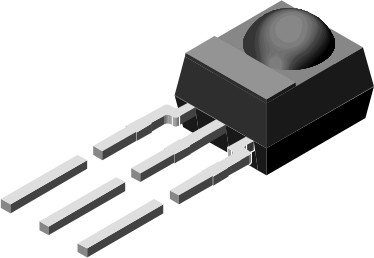
\includegraphics[width=0.4\textwidth]{Figures/TSDPSensor.jpg}
  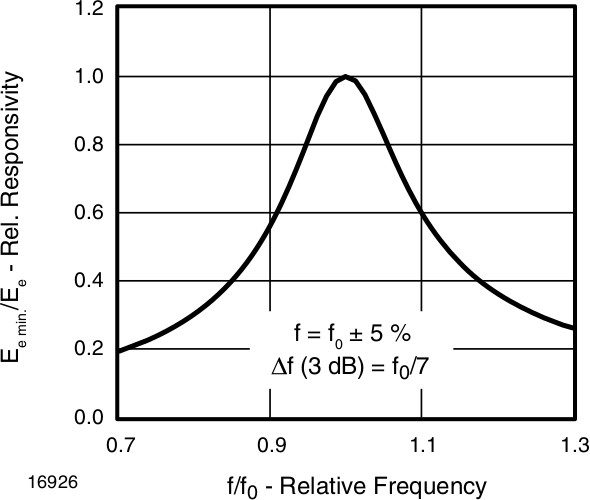
\includegraphics[width=0.4\textwidth]{Figures/TSDPFrequencyResponse.jpg}
  \caption{The TSDP34... sensor (left) and its frequency response (right).}
\end{figure}

Together with the sensor, Vishay also supplies a LED, TSAL6200, which we will use for the emitter (as it shines at 940nm wavelength, the optimal wavelength of the receiver). We now have our detection system.

This is one important thing to understand: due to the binary nature of the sensor, we cannot know the distance from the light source (we just know that there is one in the field of view of the sensor). This is quite intrinsically due to the fact that there is not link between the emitter and the receiver (distances can be measured by a telemeter laser, but in this case the emitter and receiver are located in the same device, so typically a phase shift can be computed, from which one can compute the distance). The consequence is that this system will only give the angular position of the emitter, in a certain slot. However, when designing this beacon, we felt that having a full field of view, with no blind spot, was more important that the true distance (if we know that we have a robot on our right, we don't really care about the distance, we just want to avoid going right). Beside, one can have an approximation of the distance by taking into account the fact that, the closer the object, the more sensors will activate. This hypothesis in fact proved to be rather accurate: one can definitely define a threshold, where for instance only one sensor activating would mean the robot is between 40 and 60cm away, while more that 3 sensors indicates less than 40cm (which, given the size of the robot, definitely means we should not try to go toward this robot !). This limitation can also be partially compensated by adding more conversational distance sensors (IRs or ultrasonic) to the front of the robot for example, to get a more precise measurement if the robot is moving toward an obstacle. Note that the typical distances included here depend on the tuning of the emitter: a potentiometer on this board regulates the current in the LEDs, and thus the detection distance.

\subsection{LED signal}

We know that the LED will be pulsed at the receiver frequency. Can we just make the LED emit continuously, and have the receiver listen for it ? The answer is no, because of internal filtering of the TSDP34... Before we go into technical details, one may also note that it is desirable to have some form of communication protocol on top of this (for instance, listen only to pulses of a given length). This makes the design even more robust to outer perturbations: even if there is a light source (another beacon?) at the same frequency, it most likely won't be using the same pulse lenght for its signal. This makes false positive almost impossible (but not false negative: if someone is shinning a continuous light at the right frequency, we won't see our pulse).

This sensor was designed with the idea in mind that the remote controller would try to send a serial signal to the TV, not a continuous pulse. To enhance transmission, Vishay integrated what they call an automatic gain control (AGC) circuit. This circuit is responsible for "locking" on a signal once it is detected, as mentioned in the datasheet: \emph{When a data signal is applied to the receiver in the presence of noise, the sensitivity of the receiver is automatically reduced by the AGC to insure that no spurious pulses are present at the receiver’s output.} The consequence of this is an hysteresis phenomenon: on my first prototype, one would for instance need to bring the emitter as close as 30cm to the receiver to begin detection, but could bring it 2m away and still have detection ! This was because I had overlooked this issue, which is only rapidly mentioned in the datasheed (for more information, have a look at Vishay application note, present in the Documentation folder), and chosen the \emph{AGC3 FOR NOISY ENVIRONMENTS} version, for more robustness. I then changed to the \emph{AGC1 FOR LOW NOISE ENVIRONMENTS} while redesigning the signal, which removes (almost) completely this phenomenon.  I thus strongly suggest you use the TSDP34138 and TSDP34156 sensors, and not their TSDP34338/TSDP34356 counterpart.

Figure \ref{fVishayApplication} from the application note gives the response of the AGC1 filter. The X axis gives the pulse bust lenght, in number of cycles (i.e. number of iterations of the 57.6kHz signal). Obviously one can only send bytes atop a 57.6kHz frequency at a frequency much lower than 57.6kHz: these sensors were designed for 7800bps UART communication. The Y axis gives the duty cycle of the pulse. Anything below the blue curve passes, and is recieved, while anything above the green curve is suppressed.

\begin{figure}[h]
  \centering
  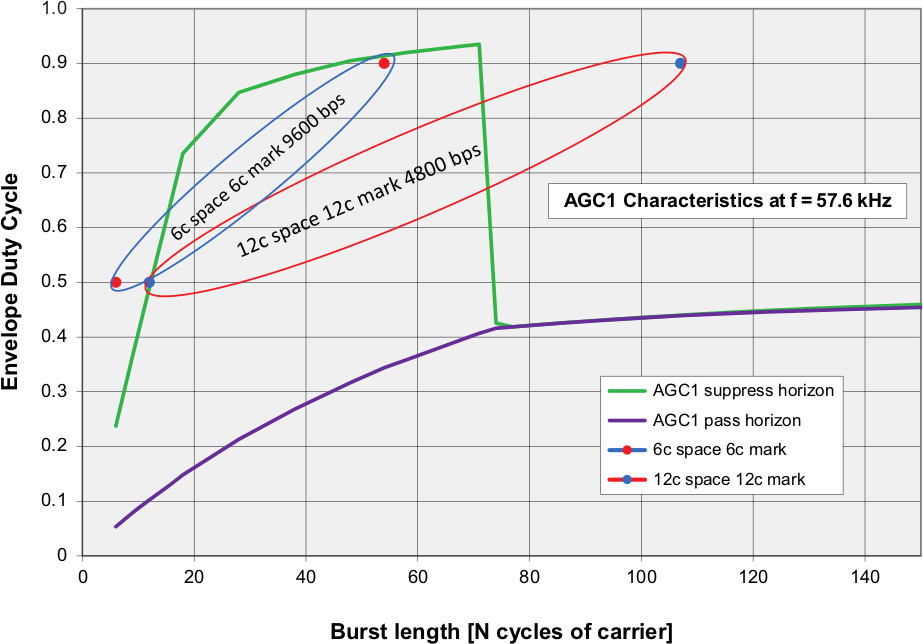
\includegraphics[width=\textwidth]{Figures/AGC1.jpg}
  \caption{AGC1 filter response.}
  \label{fVishayApplication}
\end{figure}

As one can see, continuous signals are always suppressed, while single pulse will always pass. The problem is what happens in between: in this (large) hysteresis region, the behavior depends on the history: if we travel from the lower regions, it will continue to pass, while if we travel from the higher regions, it won't pass. 

What is draw on the diagram are the regions were various UART sequences are placed. However, we won't be using UART here (unlike what is done in totofweb), because the result would be quite slow. Indeed, most microcontroller only have one serial port, which means that we will have to read the receivers one by one. Going around the whole beacon would thus take some time. To be faster, we can instead send a single pulse, whose length we will read using interrupts. This gives a simpler and faster protocol. On this diagram, a periodic pulse is simply a point, defined by its pulse length and duty cycle. The hysteresis phenomenon I described was linked to the fact that, at first, this point was situated in the hysteresis region. What as guess was happening was that, as we got closer, some signal would end up passing the AGC (it only applies a gain, but probably can't completely kill a signal). Then the AGC would actually "latch" on that signal and remain active as we go further away, until the signal is completely lost, at which point the AGC goes to rest again (what isn't mentioned in this diagram is that this AGC is a dynamic filter, changing state with time).

To remove the hysteresis, we thus want our point to be below the blue line. To be as fast as possible, we want a pulse as short as possible with a low duty cycle (this is because the blue curve's slope is lower than one: by sending a pulse twice longer, we don't multiply the duty cycle by 2, thus the resulting period is higher). The minimum pulse length is 6 carrier cycles: the corresponding duty cycle is then around 5\%. I wanted the same signal for both 38.4kHz and 57.6kHz receivers (as both will be used, see below): taking into account microcontroller constraints, I ended up with the following signal: a single pulse of 192 microseconds among a periodic signal of 5ms. This gives a duty cycle of 4\% and 7.4 carrier cycles at 38.4kHz, 11 at 57.6kHz. Thanks to this, the AGC no longer triggered, and we had a more stable detection, in only 5 milliseconds per sensor. If you look at the same curve for AGC3, you will notice that the blue curve is significantly lower, meaning that, to get the same effect, we would have needed a lower duty cycle, and thus a longer signal period.

\subsection{Sensibility to other IR beacons}

This is one final thing to consider in the design: we've seen that this sensor is sensible only to a specific frequency, thus achieving our goal of ignoring ambient light. But what if the other team happens to also use plused IRs ? Worst, what if they happen to use the exact same frequency ? This might look unlikely, given than for now few teams used such IR beacons. But it's not unlikely that they were inspired from the same design as I (and in the future, several team may be building from this very document), which could be a conflict. Besides, looking at these sensors, I realised that the choice of frequency was extremely poor. Overall, Vishay seems to be the dominant player in this sensor system, and currently most of their sensors are built using de facto standard frequencies of 38.4kHz or 57.6kHz. This problem was partially identified in the totofweb design, where the author exaplains that these two frequencies tend to be "crowded". For this reason, he had chosen a sensor working at 455kHz, but Vishay is no longer manufacturing it (I guess that against the development of wifi and bluetooth, high-speed IR transmission had little future).

Thus, we feared that we might meet a team which operates at the same frequency as us, and that their emitter, placed on top of our receiver, would "blind" it. Either the receiver could be constantly active, thus blocking the robot from the start (it would believe to be surrounded), or on the contrary, given that the pulse they send would be unlikely to match ours, the robot would ignore it and, as both signals mix, would also ignore our own beacon (the sum of both signals would result in pulse not longer being of the desired length), and thus be blind. Whatever happens, it would be bad ! To prevent this, the simplest solution appears to have the ability to change on the fly the frequency ! That way, we can simply ask the other team before the match what frequency they are using (or test it if they don't know), and change it if we use the same. This is quite easy for the emitter (it's the same LED, we just change the control signal sent by the microcontroller). For the receiver, as the filter are fixed for a given version, it requires soldering twice as many receiver: every "odd" receiver would work at 38.4kHz (TSDP341380, and every even one at 57.6kHz (TSDP34156).

 We might have actually overestimated this problem, as in fact, if we place our own beacon on top of the receiver, it does not see it (light is emitted parallel to the receiver, not towards it). One could imagine some form of mechanical cap isolating it from the other beacon... Still, we have not guarantee that the issue would not appear with another beacon design, where perhaps they use stronger LEDs (reflection of the light on the wall can make it possible, if enough current is send through the LEDs, to "see" the receiver even without direct exposition). 

\section{Emitter design}

The emitter overall consist of a ring of IR LEDs. In order to regulate the LED brightness, needed to adjust detection distance, an adjustable current regulator is used, using an operational amplifier and a transistor. A potentiometer is used to regulate the current. Note that the current design (potentiometer value and resistor placed in series with the LEDs) is made to allow a current of up to 100mA in the LEDs, the maximum admissible. This was done because I had no real idea of how much current would be needed, though I knew I probable wouldn't need as much (Vishay claims ranges up to 32m with this). In practice the current sent is lower than 10mA, so the design could be updated (no need for a 2W resistor - potentiometer value could be changed to give a better tunning range).

We now need to generate the voltage input signal for the current regulator. We need both a carrier, whose frequency should change between 38.4kHz and 57.6kHwz, and the pulse we wanted. For this, an ATTiny85 is used: it is small (only 8 pins, the minimum for a microcontroller), and can be programmed easily, by an Arduino for example. Changing the input signal is then as easy as writing code (no need for new electronics). Note that on board programming was not implemented, but I guess this could be added to the board (I found it just as easy to remove the chip, so as not to have to deal with wiring, but this might lead to pins breaking).

Since we need precise timing, the signals are not generated using software calls to change the pin state, but directly using the timers of the microcontroller. One pin thus generates the carrier, and the other the pulse: the precision is then that of the ATTiny clock, a few percents. The signals are then electronically combined using an AND gate. Note that the pulse generating pin was purpusefully choosen to be the UART TX pin of the microcontroller, to enable UART pulse writing if one wants to try this instead.

To complete the design, a voltage regulator is responsible for providing 5V to the microcontroller. A (visible) LED blinks in a heartbeat fashion to indicate that the code was properly flashed and is running. Finally, a switch allows to choose the IR frequency.

\section{Receiver design}

The receiver will consist of many IR sensors connected to a microcontroller, that will relay the processed information to the outside through a simple I2C communication. In order to speed up detection, one wants to be able to read many sensors at once. The limitations resides in the number of independent interrupts the microcontroller can provide: indeed, detection consists in detecting accurately the lenght of the input pulse, thus the need for interrupts. I choose an ATTiny 841, which features 3 independents interrupts compatible with its use as an I2C slave. Note that this microcontroller could also be used for UART transmission, but this would require a change in board wiring to output the right port.

Thus, 3 IR sensors can be read at the same time: the number of sensors will be a multiple of 3. As we decided to alternate between 38.4kHz and 57.6kHz sensors, we will in fact need muliples of 6. In the end, 18 sensors were placed on the board (size limitation couldn't really tolerate 24 sensors), 9 for each frequency. This means one sensor every $40^\circ$. Only 3 cycles are needed to do a full detection: at 5ms per sensors, this theoretically means only 15ms. The current code takes twice longer, as we wait 10ms on each sensor: this gives more stable readings, in the case where the sensor misses a single pulse. Three mult2iplexers are used to connect the various interrupt pins to the sensors ; once more, a heartbeat LED and frequency switch is integrated. All the components can work from either 3.3V or 5V.

\begin{figure}[h]
  \centering
  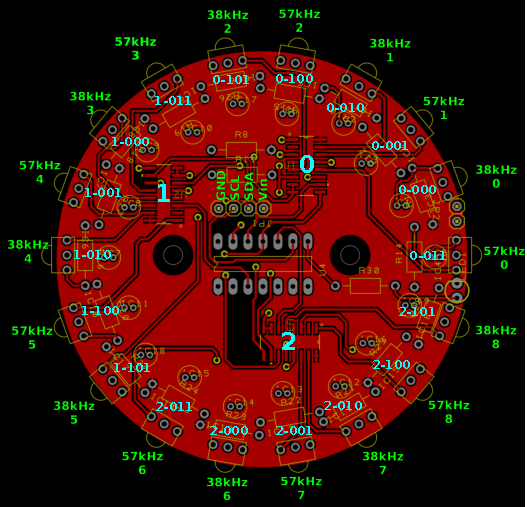
\includegraphics[width=0.7\textwidth]{Figures/IC_Documentation_Reciever.pdf}
  \caption{Annotated receiver PCB giving sensor placement (green) and multiplexer indexing (blue).}
  \label{fReceiverDoc}
\end{figure}

Figure \ref{fReceiverDoc} gives an annotated version of the board. The numbers in blue relate to the multiplexer indexing, and is only useful from a coding point of view. In green, we see how the sensors are to be placed, and what number they are given in the code. In I2C, one can ask mainly for raw sensor information, in which case the current value of sensors 0 through 8 are returned (hence the numbering in green), or for direct robot position. The microcontroller indeed integrates a grouping algorithm, where the two largest groups of continuous sensors seeing an emitter are considered as a robot, whose central position and size is returned. For complete information on the I2C registers, look at the document IR\_I2C\_Registers.pdf in the Documentation folder.

\end{document}
